\documentclass[conference]{IEEEtran}
\IEEEoverridecommandlockouts

\usepackage{cite}
\usepackage{amsmath,amssymb,amsfonts}
\usepackage{algorithmic}
\usepackage{graphicx}
\usepackage{textcomp}
\usepackage{xcolor}

\begin{document}

\title{Quantifying Gentrification Technical Report}

\author{\IEEEauthorblockN{Amy Boncelet}
\IEEEauthorblockA{\textit{Jacobs Technion-Cornell Institute} \\
\textit{Cornell Tech}\\
New York City, United States of America \\
ajb347@cornell.edu}
\and
\IEEEauthorblockN{Matthew Shen}
\IEEEauthorblockA{\textit{Jacobs Technion-Cornell Institute} \\
\textit{Cornell Tech}\\
New York City, United States of America \\
mds377@cornell.edu}
\and
\IEEEauthorblockN{Thomas Wallace}
\IEEEauthorblockA{\textit{Jacobs Technion-Cornell Institute} \\
\textit{Cornell Tech}\\
New York City, United States of America \\
tw526@cornell.edu}
}

\maketitle

\begin{IEEEkeywords}
Urban Technology, Urban Data, Data Science, Information Systems
\end{IEEEkeywords}


\section{Analysis}

\subsection{How we defined gentrification}
In order to define gentrification, we looked at six different metrics. A change in any of these metrics would mean an increase or decrease in gentrification. A summary of these metrics and how their change corresponds to gentrification can be seen in Table~\ref{gen_metrics}.

\begin{table}[htbp]
\caption{Gentrification Metrics}
\begin{center}
\begin{tabular}{cc}
\hline\hline
\textbf{An increase in this metric =} & \textbf{An increase in this metric =} \\
\textbf{Increase Gentrification} & \textbf{Decrease Gentrification} \\
\hline
\% White Population* & Median Age                                   \\
Median Income        & \% Foreign Born(Non-US Citizen)*              \\
\% Bachelor's Degree* & \\
\% Median Rent &\\
\hline\hline
\multicolumn{2}{l}{Per Capita Calculation Required*}
\end{tabular}
\label{gen_metrics}
\end{center}
\end{table}

These metrics were selected based on \cite{b1}, \cite{b2}, \cite{b3}, and \cite{b4}

\subsection{Project Scope}
We looked at information between 2011 and 2019 from the US Census Bureau. 2011 was the starting point because it was the first year with available data. 2019 was the end point to avoid any atypical demographic changes due to the 2020 COVID-19.

ZCTA5 values were used as the baseline, because they remain relatively constant over time, which meant that our baseline would be consistent.

\subsection{Methodology}

\subsubsection{Year Organization}
The data that we used from the US Census Bureau was collected from four different surveys. These different surveys can be seen in Table~\ref{surveys}.
\begin{table}[htbp]
\caption{US Census Bureau Surveys}
\begin{center}
\begin{tabular}{cc}
\hline\hline
\textbf{Survey Code} & \textbf{Survey Description} \\
\hline
DP05 & ACS Demographic \& Housing Estimates\\
S1901 & Income in the Past 12 Months\\
DP02 & Selected Social Characteristics\\
DP04 & Selected Housing Characteristics\\
\hline\hline
\end{tabular}
\label{surveys}
\end{center}
\end{table}
Each survey came in separate files for each year. These data sets were merged into one file for each individual year. 

\subsubsection{Column Metadata}
Column metadata changed for some of our variables over the years. We determined how the column names changed with each year to ensure we grabbed the correct data set for each year. The relevant columns used can be found in Appendix~\ref{app_A}.

Once all the columns were renamed we subset the data to only include the ZCTA5s, the data in Table~\ref{gen_metrics}, and the total population.

\subsubsection{Cleaning Data Types}
Some of the census data was presented as strings. In order to process the data, we either converted the data to a float/integer or removed the data (if it was not needed).

We also found that the ZCTA5 data was in the format of "ZCTA5 00000". To allow for easier querying we striped the "ZCTA5 ".

We also found that some ZCTA5 values did not have an associated population. This was likely due to new office buildings that have independent ZCTA5 values and no residents. We removed these rows that did not have a population.

The final data cleaning measure was to subset the ZCTA5s to only include ones in NYC.

\subsubsection{Interpolating Missing Data}
Once the data for each year was cleaned and subset, we reviewed for any missing data in the gentrification factors. We filled any missing data by interpolating with the nearby ZCTA5 values. We used interpolation rather than filling missing data with the city-wide mean because we can make the assumption that ZCTA5 values near each other would have similar values.

\subsubsection{Calculate change over time}
The next step was the look at how our different metrics changed over time. To do this, we merged the cleaned data sets from 2011 and 2019 on the ZCTA5s and then found the difference between 2011 and 2019. Next, we transformed the metrics in Table~\ref{gen_metrics} that decrease gentrification into negative numbers. This ensures that an increase in any of our gentrification factors results in a lower gentrification score.

\subsubsection{Normalize data}
We finally normalized the data with Equation~\ref{norm}.
\begin{equation}
\frac{x-\mu}{\sigma}\label{norm}
\end{equation}
In Equation~\ref{norm} $x$ is the value we are changing, $\mu$ is the mean of the series that data set, and $\sigma$ is the standard deviation of the series that data set. This normalization ensured that the magnitude of the values did not effect the gentrification metric.

\subsubsection{Creating the Gentrification Metric}
Now that our data is normalized, we created our gentrification metric by adding all the values in Table~\ref{gen_metrics} for each ZCTA5.

\section{Results}
The gentrification metric was plotted with respect to each zip code. This visualization can be seen in Appendix~\ref{app_b}.

\begin{thebibliography}{00}
\bibitem{b1} A. Owens and J. Candipan, ``Racial/Ethnic Transition and Hierarchy Among Ascending Neighborhoods'' \textit{Urban Affairs Review}, vol. 55, no. 6, Apr. 2018. Accessed: Dec. 4, 2022. doi: https://doi.org/ 10.1177/107808741877081. [Online]. Available: https://journals.sagepub.com/doi/10.1177/1078087418770810

\bibitem{b2} M. Cohen and K. L. S. Pettit, "Guide to Measuring Neighborhood Change to Understand and Prevent Displacement," \textit{National Neighborhood Indicators Partnership(NNIP)}, Boston, MA, 2016. Accessed Dec. 4, 2022. [Online]. Available: https://www.urban.org/sites/default/files/publication/100135/guide\_to\_ measuring\_neighborhood\_change\_to\_understand\_and\_prevent\_ displacement.pdf

\bibitem{b3} T. Buffel and C. Phillipson, “Ageing in a Gentrifying Neighbourhood: Experiences of Community Change in Later Life,” \textit{Sociology}, vol. 53, no. 6, Apr. 2019. Accessed: Dec. 4, 2022. doi: https://doi.org/10.1177/0038038519836848. [Online]. Available: https://journals.sagepub.com/doi/full/10.1177/0038038519836848

\bibitem{b4} J. Hwang, “Immigration is an important dimension in how we understand gentrification across US cities,” \textit{London School of Economics}, Oct. 2015. Accessed: Dec. 4, 2015. [Online]. Available: https://blogs.lse.ac.uk/usappblog/2015/10/21/immigration-is-an-important-dimension-in-how-we-understand-gentrification-across-us-cities/ 


\end{thebibliography}

\clearpage
\appendix[Column Names Over Time]\label{app_A}
\begin{table}[htbp]
\caption{Bachelor's Degree}
\begin{center}
\begin{tabular}{cc}
\hline\hline
\textbf{Year} & \textbf{Code} \\
\hline
2011 & DP02\_0064E \\
2012 &  \\
2013 &  \\
2014 &  \\
2015 &  \\
2016 &  \\
2017 &  \\
2018 &  \\
\hline
2019 & DP02\_0065E \\
\hline\hline
\end{tabular}
\end{center}
\end{table}
\begin{table}[htbp]
\caption{Foreign born, not a US Citizen}
\begin{center}
\begin{tabular}{cc}
\hline\hline
\textbf{Year} & \textbf{Code} \\
\hline
2011 & DP02\_0095E \\
2012 & \\
2013 & \\
2014 & \\
2015 & \\
2016 & \\
2017 & \\
2018 & \\
\hline
2019 & DP02\_0096E \\
\hline\hline
\end{tabular}
\end{center}
\end{table}
\begin{table}[htbp]
\caption{Median Income}
\begin{center}
\begin{tabular}{cc}
\hline\hline
\textbf{Year} & \textbf{Code} \\
\hline
2011 & S1901\_C01\_012E \\
2012 & \\
2013 & \\
2014 & \\
2015 & \\
2016 & \\
2017 & \\
2018 & \\
2019 & \\
\hline\hline
\end{tabular}
\end{center}
\end{table}
\begin{table}[htbp]
\caption{White Non-hispanic}
\begin{center}
\begin{tabular}{cc}
\hline\hline
\textbf{Year} & \textbf{Code} \\
\hline
2011 & DP05\_0072E \\
2012 & \\
2013 & \\
2014 & \\
2015 & \\
2016 & \\
\hline
2017 & DP05\_0077E\\
2018 & \\
2019 & \\
\hline\hline
\end{tabular}
\end{center}
\end{table}
\begin{table}[htbp]
\caption{Median Age}
\begin{center}
\begin{tabular}{cc}
\hline\hline
\textbf{Year} & \textbf{Code} \\
\hline
2011 & DP05\_0017E \\
2012 & \\
2013 & \\
2014 & \\
2015 & \\
2016 & \\
\hline
2017 & DP05\_0018E\\
2018 & \\
2019 & \\
\hline\hline
\end{tabular}
\end{center}
\end{table}
\begin{table}[htbp]
\caption{Rent - Gross rent median price}
\begin{center}
\begin{tabular}{cc}
\hline\hline
\textbf{Year} & \textbf{Code} \\
\hline
2011 & DP04\_0132E \\
2012 & \\
2013 & \\
2014 & \\
\hline
2015 & DP04\_0134E\\
2016 & \\
2017 & \\
2018 & \\
2019 & \\
\hline\hline
\end{tabular}
\end{center}
\end{table}

\clearpage
\appendix[Gentrification Map]\label{app_b}
\begin{figure}[htbp]
\centerline{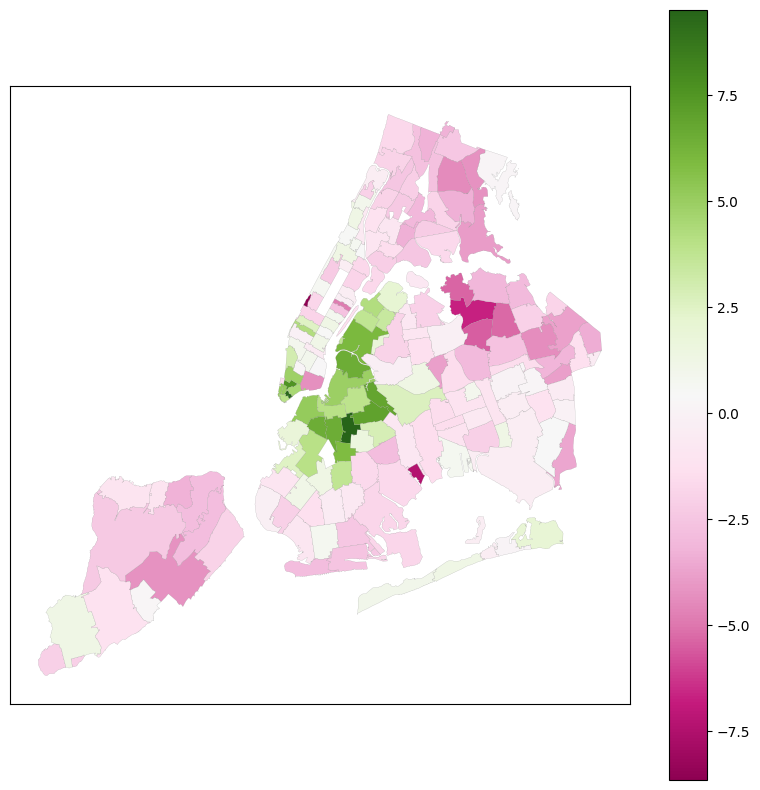
\includegraphics[width=0.45\textwidth]{images/gen_map.png}}
\end{figure}

\end{document}
